%%%%%%%%%%%%%%%%%%%%%%%%%%%%%%%%%%%%%%%%%%%%%%%%%%%%%%%%%%%%%%%%%%%%%%%%%%%%%%%%
%2345678901234567890123456789012345678901234567890123456789012345678901234567890
%        1         2         3         4         5         6         7         8

\documentclass[letterpaper, 10 pt, conference]{ieeeconf}  % Comment this line out if you need a4paper

%\documentclass[a4paper, 10pt, conference]{ieeeconf}      % Use this line for a4 paper

\IEEEoverridecommandlockouts                              % This command is only needed if 
                                                          % you want to use the \thanks command

\overrideIEEEmargins                                      % Needed to meet printer requirements.

%In case you encounter the following error:
%Error 1010 The PDF file may be corrupt (unable to open PDF file) OR
%Error 1000 An error occurred while parsing a contents stream. Unable to analyze the PDF file.
%This is a known problem with pdfLaTeX conversion filter. The file cannot be opened with acrobat reader
%Please use one of the alternatives below to circumvent this error by uncommenting one or the other
%\pdfobjcompresslevel=0
%\pdfminorversion=4

% See the \addtolength command later in the file to balance the column lengths
% on the last page of the document

% The following packages can be found on http:\\www.ctan.org
%\usepackage{graphics} % for pdf, bitmapped graphics files
%\usepackage{epsfig} % for postscript graphics files
%\usepackage{mathptmx} % assumes new font selection scheme installed
%\usepackage{times} % assumes new font selection scheme installed
%\usepackage{amsmath} % assumes amsmath package installed
%\usepackage{amssymb}  % assumes amsmath package installed
\usepackage[utf8]{inputenc}
\usepackage[T1]{fontenc}
\usepackage{graphicx}
\usepackage{amsmath}
\usepackage{amssymb}
\usepackage{bm}
\usepackage{booktabs}
\usepackage{makecell}
\usepackage{multirow}
\usepackage{subcaption}

\title{\LARGE \bf
Improving Human-Robot Teamwork in Urban Search and Rescue Through Knowledge Graph-Based Episodic Memory Learning
}


\author{Taewoon Kim$^{1}$, Emma van Zoelen$^{2}$, and Mark Neerincx$^{2}$%
\thanks{$^{1}$Taewoon Kim, HumemAI, The Netherlands
        {\tt\small taewoon@humem.ai}}%
\thanks{$^{2}$Emma van Zoelen and Mark Neerincx, TNO, The Netherlands
        {\tt\small emma.vanzoelen@tno.nl}, {\tt\small mark.neerincx@tno.nl}}%
}


\begin{document}



\maketitle
\thispagestyle{empty}
\pagestyle{empty}


\begin{abstract}
Effective human–robot teamwork demands that robots adapt on the fly to volatile, co‑evolving human behavior. In MATRX USAR simulations, performance rises when humans label and share collaboration patterns (CPs) with the robot via chat. This study aims to advance human-robot collaboration by developing an episodic long-term memory that integrates and maintains these patterns in a dedicated ontology-based Knowledge Graph (KG). We apply graph representation self-supervised learning to cluster these memories, identifying the most representative and effective experiences. Unlike previous approaches where robots start with an empty memory state, we initialize the robot’s memory with these insights, enabling it to retain knowledge. On 160 trials, seeding the robot with a single, automatically chosen CP lifts rescue success from 25.7\% to 41.3\% and cuts average task time by 283s.
\end{abstract}

% Uncomment the following to link to your code, datasets, an extended version or similar.
% You must keep this block between (not within) the abstract and the main body of the paper.
% \begin{links}
%     \link{Code}{https://aaai.org/example/code}
%     \link{Datasets}{https://aaai.org/example/datasets}
%     \link{Extended version}{https://aaai.org/example/extended-version}
% \end{links}

\section{Introduction}
\label{sec:introduction}


\begin{figure}[tb]
\centering
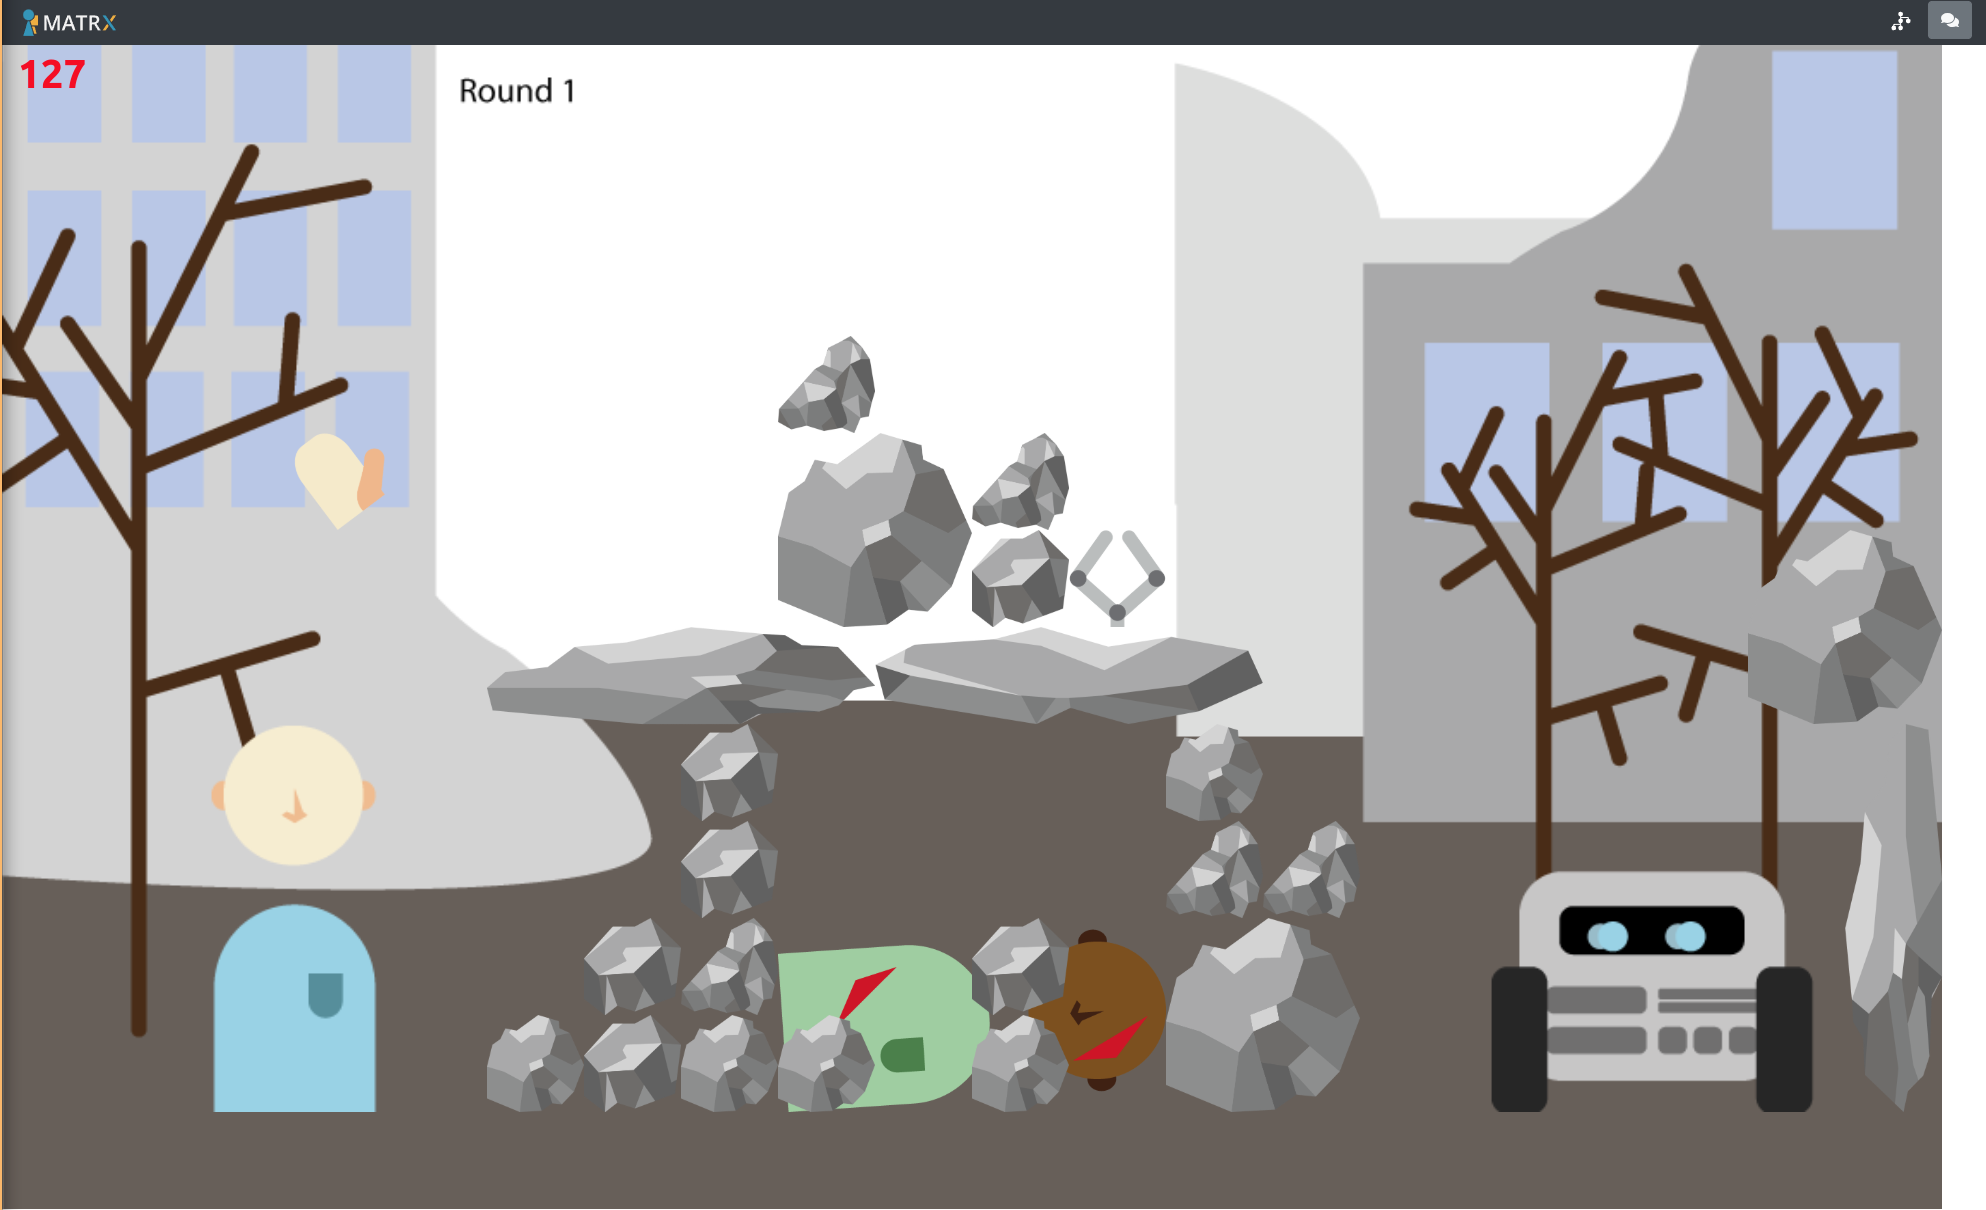
\includegraphics[width=\columnwidth]{figures/usar.png}
\caption{A screenshot of the MATRX USAR simulation. The human user is shown on the left, while the robot is on the right. In the upper right corner, users can click icons to define a collaboration pattern (CP) or open the chat interface.}
\label{fig:usar-main}
\end{figure}


\begin{figure}[tb]
\centering

\begin{subfigure}[b]{\columnwidth}
    \centering
    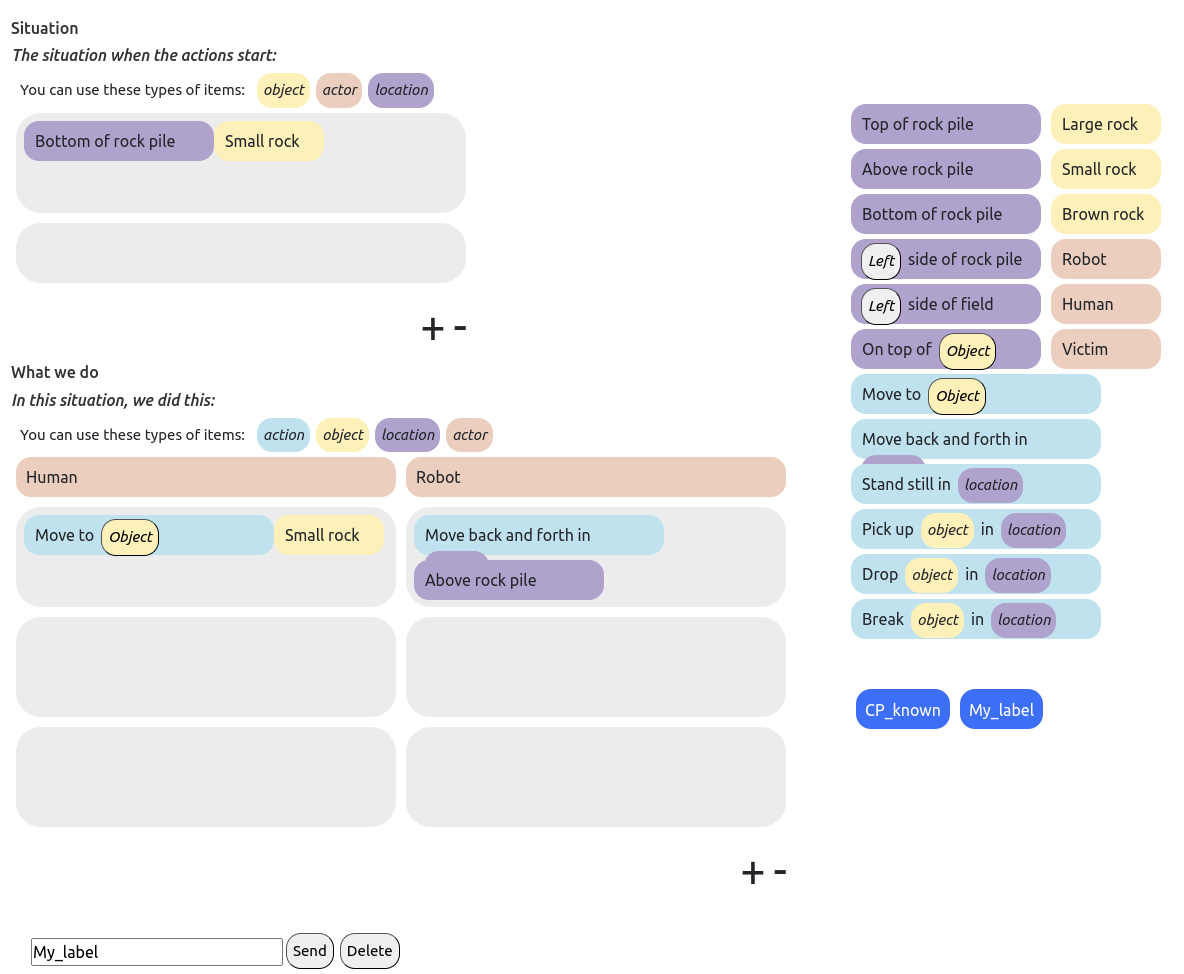
\includegraphics[width=\columnwidth]{figures/usar-cp.png}
    \caption{Users can drag and drop boxes (representing objects, actors, and locations) to document the emergent CPs they observe with the robot.}
    \label{fig:usar-cp}
\end{subfigure}

\vspace{1em}

\begin{subfigure}[b]{\columnwidth}
    % We manually create two columns within this subfigure:
    \begin{minipage}[b]{0.49\columnwidth}
        \centering
        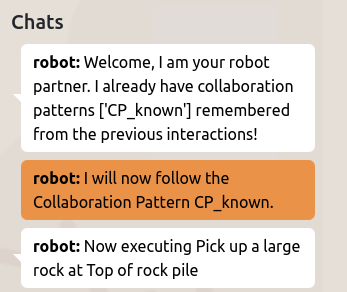
\includegraphics[width=\linewidth]{figures/usar-chat.png}
        % You can place a label here if needed, but typically
        % you'll label the entire subfigure (b) rather than just the image.
    \end{minipage}
    \hfill
    \begin{minipage}[b]{0.49\columnwidth}
        \small
        This chat interface enables the robot to communicate updates
        and inform human users about ongoing events.
    \end{minipage}

    \caption{The chat interface.}
    \label{fig:usar-chat}
\end{subfigure}

\caption{User interaction features in the MATRX USAR environment.
(a) The CP interface. (b) The chat interface.}
\label{fig:usar-interaction}
\end{figure}



Industrial robots usually work in static settings with little human contact~\cite{IFR2023}, but labour shortages and hazardous tasks are driving a shift toward teammate‑style autonomy~\cite{MarketsandMarkets2024}. For example, in disaster response, assistive robots are being developed to assist rescue teams by navigating debris, locating survivors, and delivering supplies in hazardous environments~\cite{Moosavi2024}.

Despite their potential, assistive robots face significant challenges in adapting to human partners. Unlike traditional robots operating in controlled environments, assistive robots must interpret human intentions, adjust to dynamic situations, and learn from past interactions. Human behavior is dynamic and variable, requiring assistive robots to process ambiguous cues, coordinate effectively, and refine their decision-making over time. These complexities make real-time adaptation difficult, highlighting the need for learning mechanisms that enable assistive robots to build and utilize memory from prior experiences.

One approach to studying human-robot collaboration is the MATRX Urban Search and Rescue (USAR) environment~\cite{matrx_2023,vanZoelen2021}, a virtual simulation where a collaborative robot and a human work together to rescue victims. Previous studies have demonstrated that robots in this setting can adapt to human behavior over time, improving teamwork efficiency. Notably, allowing human participants to specify collaboration patterns (CPs) and communicate through a chat interface has been shown to enhance coordination, leading to more effective rescue operations~\cite{10.1145/3434074.3446354,vanZoelen2021,vanZoelen2022}. In this context, CPs are defined as human-robot actions conditioned on situations (See Fig~\ref{fig:usar-cp}).

Shared memory has long been recognized as a key element in fostering mutual understanding between humans and robots~\cite{Miraglia2024Shared}. Building on this concept, we leverage past experimental data as episodic long-term memories that capture previous human-robot collaborations~\cite{https://doi.org/10.48550/arxiv.2204.01611,Kim_Cochez_Francois-Lavet_Neerincx_Vossen_2023}. To distill the most representative and effective experiences, we apply graph representation learning to cluster these episodic memories. Rather than beginning each episode with an empty memory state, we initialize the robot’s memory with the most representative episodic memory at the start of every experiment. This augmentation equips the robot with valuable collaborative insights, ultimately enhancing its adaptation speed and overall teamwork efficiency.

To summarize, our main contributions are as follows:

\begin{itemize}
    \item \textbf{Knowledge Graph--Based Representation:} We convert existing collaboration patterns (CPs), originally stored in TypeDB, into a property graph using JanusGraph. This enables better visualization, efficient querying with Gremlin, and native support for edge and node properties, making it well-suited for relationship modeling and graph-based learning.
    
    \item \textbf{Self-Supervised Graph Learning:} We show that self-supervised graph learning allows for learning meaningful representations of CPs, which can then be used for clustering to identify the most relevant collaboration patterns.


    \item \textbf{Memory Initialization Yields Gains:} Pre‑loading the best‑in‑cluster CP raises success by 60.7\% and reduces the average task time by 283s.
        
\end{itemize}


\section{Background}
\label{sec:background}

\subsection{MATRX Urban Search and Rescue (USAR)}
\label{sec:usar}


The MATRX Urban Search and Rescue (USAR) environment~\cite{matrx_2023,vanZoelen2021} simulates a USAR scenario where a collaborative virtual robot and a human must work together to rescue a victim. Figure~\ref{fig:usar-main} provides an example screenshot of the environment, while Figure~\ref{fig:usar-interaction} illustrates the features of the user interface used for human-robot communication. The CPs were originally stored in TypeDB~\cite{typeql2024}, which uses an entity-relation model for human-robot interactions. 

The participants begin with a practice round, followed by eight real rounds of varying difficulty. They can define any CPs they find necessary, which will remain available throughout all rounds unless they choose to modify or remove them.

\subsection{Knowledge Graphs (KGs)}
\label{sec:kg}

A KG is a directed graph $\mathcal{G} = (\mathcal{V}, \mathcal{R}, \mathcal{E})$, where $\mathcal{V}$ represents entities, $\mathcal{R}$ denotes relations, and $\mathcal{E} \subseteq \mathcal{V} \times \mathcal{R} \times \mathcal{V}$ consists of edges that define the relationships between entities. Each edge $(v_i, r_k, v_j)$ indicates that a relation $r_k$ exists from entity $v_i$ to entity $v_j$~\cite{10.1145/3447772}.

KGs are typically implemented using one of two major models: Resource Description Framework (RDF) graphs~\cite{Lanthaler:14:RCA} and property graphs. RDF-based KGs represent data as triples \texttt{(subject, predicate, object)}, facilitating semantic reasoning and interoperability across different systems. For example:

\begin{quote}
    \texttt{(:Alice, :knows, :Bob)}
\end{quote}

This structure represents the fact that ``Alice knows Bob'' but does not directly store additional details such as when or how they met. 

In contrast, property graphs allow both nodes and edges to have attributes, making them more expressive for complex relationships. In a property graph model, the same knowledge can be represented as:

\begin{quote}
    \texttt{(Alice)-[knows \{since: "2020", location: "Amsterdam"\}]->(Bob)}
\end{quote}

Here, the edge \texttt{knows} has properties such as \textit{timestamp} \texttt{(since: "2020")} and \textit{location} \texttt{(location: "Amsterdam")}, which provide richer contextual information. 

In this work, we opted for a property graph model using JanusGraph~\cite{janusgraph_2024} due to its better visualization support, efficient querying with Gremlin, and native support for edge and node properties, which are crucial for modeling CPs in our scenario.


\subsection{Graph Neural Networks (GNNs)}
\label{sec:gnn}

GNNs are deep learning models designed for graph-structured data~\cite{4700287}. A graph is represented as $\mathcal{G} = (\mathcal{V}, \mathcal{E})$, where $\mathcal{V}$ is a set of nodes and $\mathcal{E}$ is a set of edges connecting these nodes. Nodes and edges can have associated features, denoted as $x_v$ and $x_{uv}$, respectively.

Graph Convolutional Networks (GCNs) extend traditional convolution operations to graphs by updating each node's feature representation based on its neighbors:
\[
\bm{g}_v^{(k)} = f\left( \sum_{u \in \mathcal{N}(v)} \bm{W}^{(k)} \bm{g}_u^{(k-1)} \right)
\]
where \( \bm{g}_v^{(k)} \) represents the feature vector of node \( v \) at the \( k \)-th layer, \( \mathcal{N}(v) \) denotes the neighbors of node \( v \), \( \bm{W}^{(k)} \) is the weight matrix for the \( k \)-th layer, and \( f \) is an activation function. This spatial approach focuses on aggregating information from local neighborhoods, differing from the spectral methods originally proposed in~\cite{DBLP:journals/corr/KipfW16}.

GNNs are crucial for tasks involving complex relational structures, such as KG reasoning and graph representation learning.


\begin{figure}[tb]
\centering

%--------------------------------------------
% Subfigure (a) - All CPs visualized
%--------------------------------------------
\begin{subfigure}[b]{\columnwidth}
    \centering
    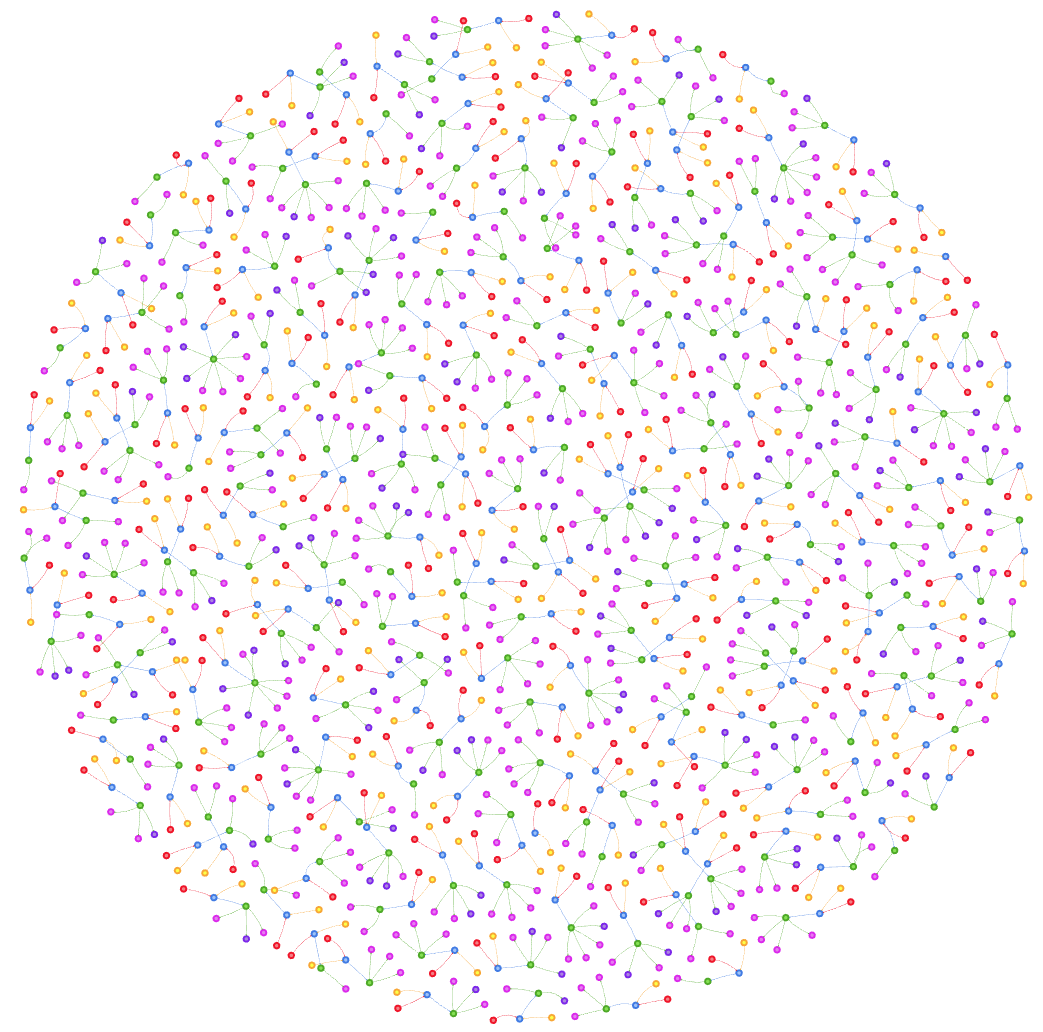
\includegraphics[width=0.7\columnwidth]{figures/g.V().png}
    \caption{A visualization of collected 209 collaboration patterns (CPs) as 209 knowledge graphs (KGs).}
    \label{fig:cps_all_visualized}
\end{subfigure}

\vspace{1em}

%--------------------------------------------
% Subfigure (b) - Example CP visualization
%--------------------------------------------
\begin{subfigure}[b]{\columnwidth}
    \centering
    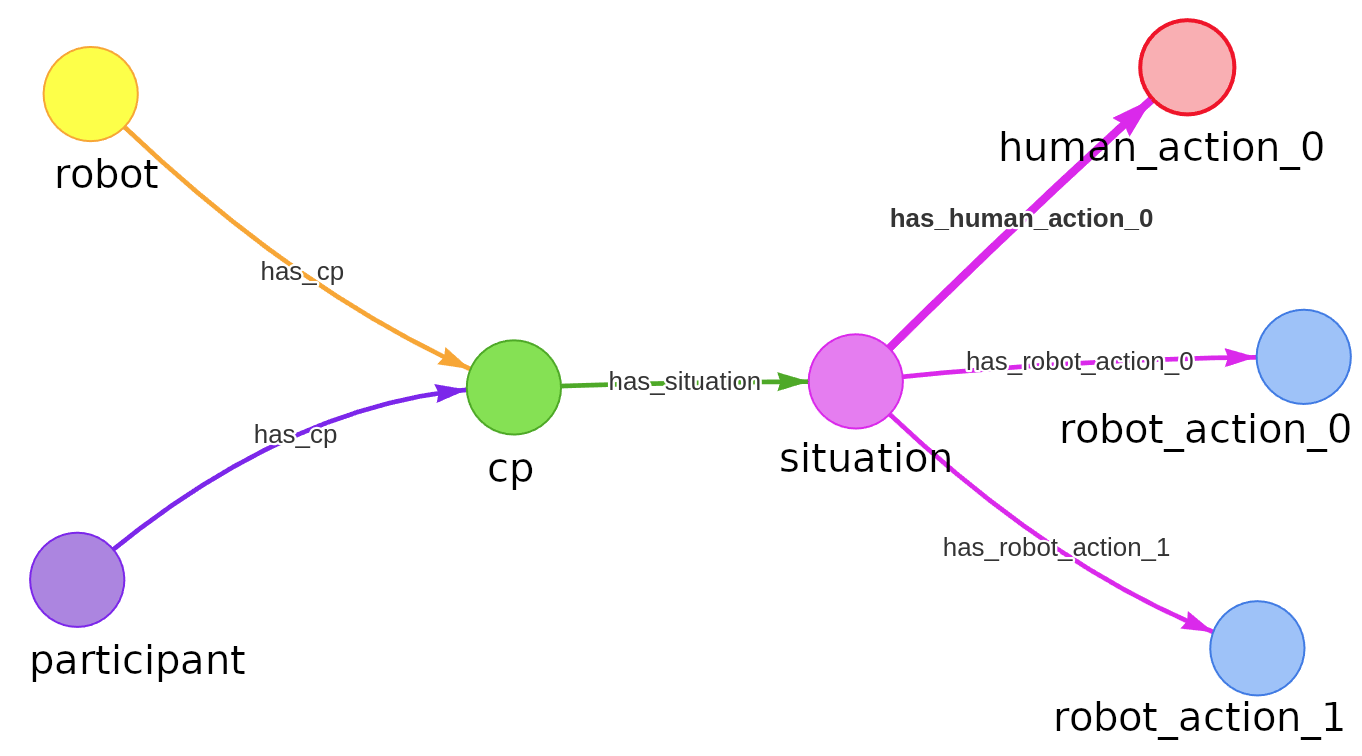
\includegraphics[width=0.75\columnwidth]{figures/cp_36.png}
    \caption{A visualization of an example CP. This knowledge graph (KG) has seven nodes: one \texttt{robot}, \texttt{participant}, \texttt{cp}, and \texttt{situation}, along with one \texttt{human\_action} and two \texttt{robot\_action} nodes. While all CPs share the same core structure, the number of \texttt{human\_action} and \texttt{robot\_action} nodes varies, as annotators define action sequences for the human and robot. A KG structure allows for this flexibility, handling dynamic node and edge counts, including varying number of \texttt{has\_human\_action} and \texttt{has\_robot\_action} edges.}
    \label{fig:cp_36_visualized}
\end{subfigure}

\caption{Visualizations of collaboration patterns (CPs) represented as knowledge graphs (KGs). (a) The entire set of 209 CPs. (b) An example CP illustrating its structural components.}
\label{fig:cp_visualization}
\end{figure}


\section{Methodology}
\label{sec:methodology}

\subsection{Ontology Engineering}
\label{sec:ontology}

Because CP graphs have variable topology, we represent them as property graphs rather than force‑fitting them into fixed‑length Euclidean vectors, thus retaining full relational context.

Our ontology defines six entity types: \texttt{robot}, \texttt{participant}, \texttt{cp}, \texttt{situation}, \texttt{robot\_action}, and \texttt{human\_action}. Each entity is represented as a node with associated properties. Relationships between entities are captured through four edge types: \texttt{has\_cp}, \texttt{has\_situation}, \texttt{has\_robot\_action}, and \texttt{has\_human\_action}, each of which can also store relevant properties. This structure provides a flexible and expressive representation of CPs, allowing detailed analysis of human-robot interactions.

From the previous studies, we have collected 209 CPs. Figure~\ref{fig:cp_visualization} visualizes them. We used the JanusGraph-Visualizer~\cite{janusgraph_2024}. 


Table~\ref{tab:cp_properties} lists the node properties of the example CP visualized in Figure~\ref{fig:cp_36_visualized}. The \texttt{cp} node properties ``time\_elapsed'', ``remaining\_rocks'', ``victim\_harm'', and ``success'', serve as round-level performance metrics. While not CP-specific, we assume that if the human-robot team performs well in a round, the CPs used contribute to that success.

\begin{table}[tb]
    \centering
    \renewcommand{\arraystretch}{1.2}
    \begin{tabular}{p{2.5cm} p{5.5cm}}
        \toprule
        \textbf{Type} & \textbf{Properties} \\
        \midrule
        \texttt{robot} &  \\
        \midrule
        \texttt{participant} & participant\_number: 4081 \\
        \midrule
        \texttt{cp} & time\_elapsed: 3000, \newline event\_time: ``2024-05-07T11:26:11'', \newline cp\_num: 36, \newline ticks\_lasted: 1917, \newline participant\_num: 4081, \newline remaining\_rocks: 32, \newline cp\_name: ``top brown'', \newline victim\_harm: 0, \newline success: false \newline round\_num: 6 \\
        \midrule
        \texttt{situation} & location: ``Top of rock pile'', \newline object: ``Brown rock'' \\
        \midrule
        \texttt{human\_action\_0} & location: ``Above rock pile'', \newline action: ``Stand still in \textless location\textgreater'' \\
        \midrule
        \texttt{robot\_action\_0} & location: ``Top of rock pile'', \newline object: ``Brown rock'', \newline action: ``Pick up \textless object\textgreater in \textless location\textgreater'' \\
        \midrule
        \texttt{robot\_action\_1} & location: ``\textless Right\textgreater side of field'', \newline object: ``Brown rock'', \newline action: ``Drop \textless object\textgreater in \textless location\textgreater'' \\
        \bottomrule
    \end{tabular}
    \caption{The node properties of the example CP.}
    \label{tab:cp_properties}
\end{table}

\subsection{Self-Supervised Learning on Graphs}
\label{sec:graph_learning}

Choosing a CP by raw score alone ignores the situational and action context that produced that score. A high-performing CP in one scenario may not generalize to others. To address this, we cluster CPs using self-supervised graph learning, capturing both performance and structural similarities. This enables us to identify the most representative and effective CPs for improved collaboration. 

Since our CPs are structured as KGs, we use a Relational Graph Convolutional Network (RGCN)~\cite{schlichtkrull2017modelingrelationaldatagraph} to learn meaningful representations. Unlike standard GNNs, RGCN incorporates edge types (e.g., \texttt{has\_cp}, \texttt{has\_human\_action}), which capture essential relational information. Through message passing, RGCN iteratively updates node features, allowing interactions between entities to shape their representations. To enable self-supervised learning, we perform node classification by adding a linear layer with softmax on top of the final RGCN layer. Each node belongs to a predefined class (e.g., \texttt{participant}, \texttt{situation}, \texttt{human\_action}), and the model learns to predict these labels. The message-passing mechanism ensures that gradients propagate beyond individual nodes, influencing their neighbors and refining the entire graph representation.

As shown in Table~\ref{tab:cp_properties}, node properties contain various features, requiring transformation into fixed-length vectors for RGCN compatibility. For \texttt{cp} nodes, we concatenate six numerical features (``time\_elapsed'', ``ticks\_lasted'', ``remaining\_rocks'', ``victim\_harm'', ``success'', and ``round\_num''), normalizing each by its maximum value to scale them between 0 and 1. For \texttt{situation}, \texttt{human\_action}, and \texttt{robot\_action} nodes, we concatenate string attributes into natural language sentences (e.g., \texttt{human\_action\_0} in the example would be ``Action: Stand still in \textless location\textgreater. Location: Above rock pile.'') and encode them using Sentence-BERT~\cite{reimers2019sentencebertsentenceembeddingsusing} to obtain numerical vector representations. Since the \texttt{cp} node vectors are shorter than the others, we apply a learnable projection matrix to transform them to the same dimensionality as the vectors for \texttt{situation}, \texttt{human\_action}, and \texttt{robot\_action} nodes.

We optimize RGCN using cross-entropy loss for node classification. Let \( f_{\theta} \) represent the entire model, including RGCN and the linear classifier. Given a CP (KG) \( \mathcal{G} \) with node features \( X \) and adjacency matrix \( A \), the predicted class distribution for a node \( v \) is:

\[
\hat{y}_v = \text{softmax}(f_{\theta}(\mathcal{G}, X, A)_v)
\]

where \( f_{\theta} \) processes the entire graph structure, and \( \theta \) includes all trainable parameters. The loss function is:

\[
\mathcal{L} = - \mathbb{E}_{(v, c) \sim \mathcal{D}_\text{train}} \left[ \log \hat{y}_{v, c} \right]
\]

where \(\mathcal{D}_\text{train}\) represents the empirical distribution of training samples, and \(C\) is the number of node classes. 

The message-passing mechanism propagates updates across the graph, refining node representations based on their connectivity. Consecutive human actions (e.g., \texttt{human\_action\_0}, \texttt{human\_action\_1}, \texttt{human\_action\_2}) and robot actions (e.g., \texttt{robot\_action\_0} to \texttt{robot\_action\_4}) are treated as distinct classes, as they represent different stages within an action sequence. Thus, we set \(C = 10\). See Figure~\ref{fig:rgcn} for a visualization of one forward pass of the RGCN-based neural network.

\begin{figure}[tb]
\centering
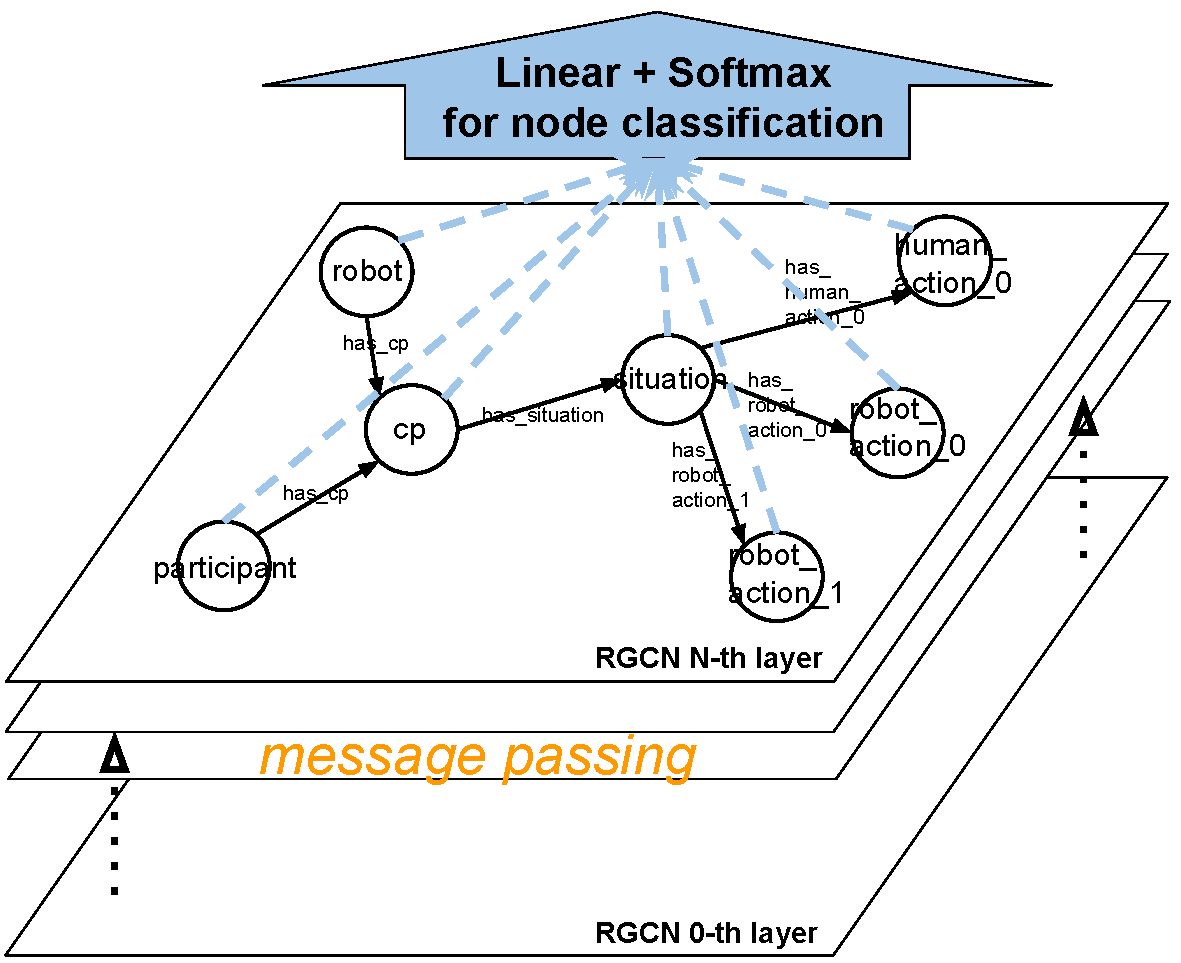
\includegraphics[width=\columnwidth]{figures/rgcn-co-learning.pdf}
\caption{A forward pass of the RGCN-based neural network. The last layer (Linear + Softmax) outputs the categorical distributions which are combined with the ground truths to compute the cross entropy loss.}
\label{fig:rgcn}
\end{figure}

After the self-supervised learning phase, we use the learned graph representations to cluster the CPs. From these clusters, we select the most representative CP, which we then use to initialize the robot’s memory. This enables the robot to start with the ``best'' episodic memory, providing it with structured prior knowledge. We then conduct human-robot interaction experiments in the same MATRX collaborative environment to evaluate the impact of this memory augmentation on task performance metrics.

\section{Experiments}
\label{sec:experiments}

The two‑layer RGCN (128,874 parameters, ReLU activations) trained for 2,000 epochs on all 209 CP graphs in a single 30s CPU run; code and hyper‑parameters are in the supplementary material, along with a recorded game play and raw data. See Figure~\ref{fig:training} for the training loss, which steadily decreases over epochs, while the accuracy increases, indicating effective learning and convergence of the model.

\begin{figure}[tb]
\centering
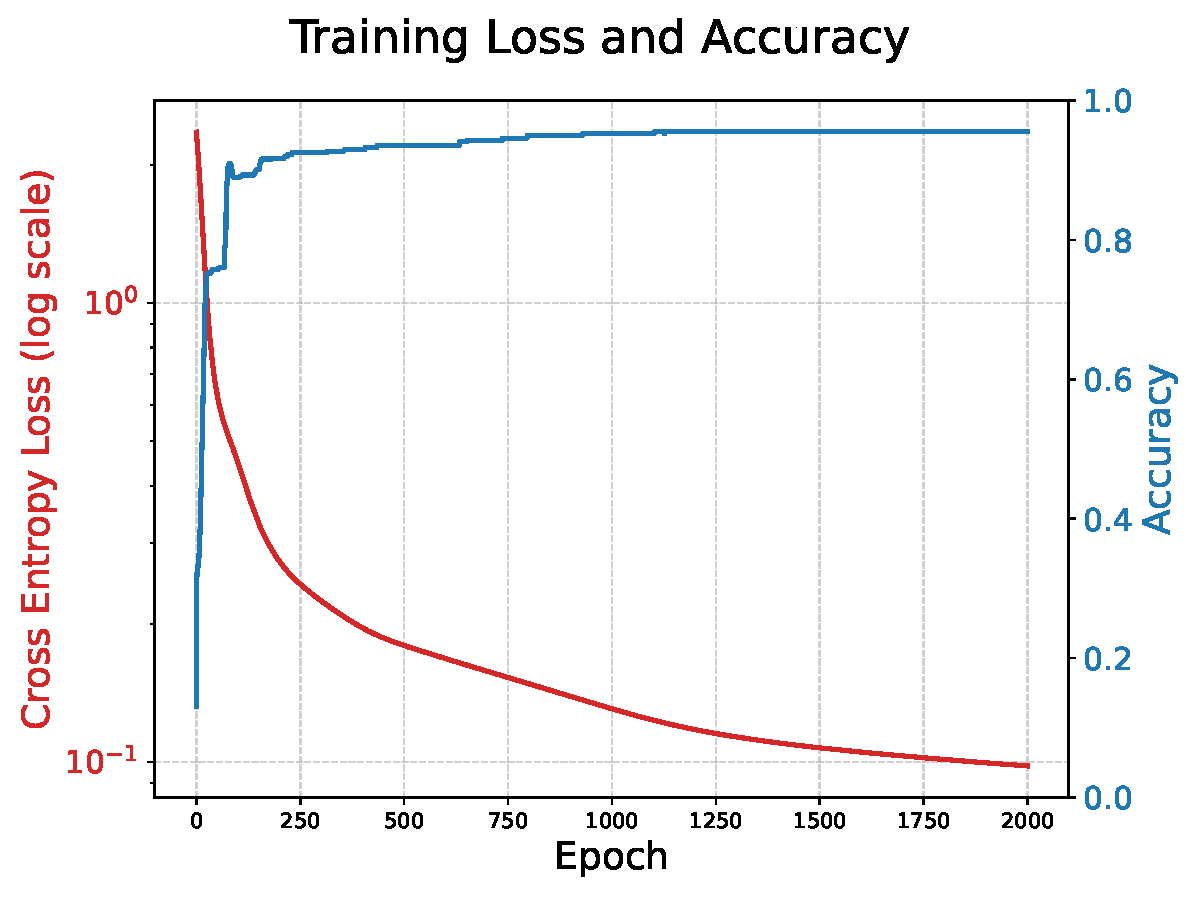
\includegraphics[width=\columnwidth]{figures/Training_Loss_and_Accuracy.pdf}
\caption{Cross entropy loss and accuracy of the training data. After 2,000 epochs, the loss dropped to 0.0948 while the accuracy went up to 95.5\%.}
\label{fig:training}
\end{figure}

After training, we obtain the final vector representation of each CP by averaging the node representations (before the classification layer) within each graph. We then apply the K-means clustering algorithm to group CPs based on Euclidean distance. Figure~\ref{fig:cluster} illustrates the clusters before and after training, with t-SNE~\cite{NIPS2002_6150ccc6} used for 2D visualization. It can be seen that the self‑supervised GNN learns the meaningful representations to cluster CPs. The number of CPs in the clusters are 62, 38, 36, 30, and 43, respectively.

\begin{figure}[tb]
\centering

\begin{subfigure}[b]{\columnwidth}
    \centering
    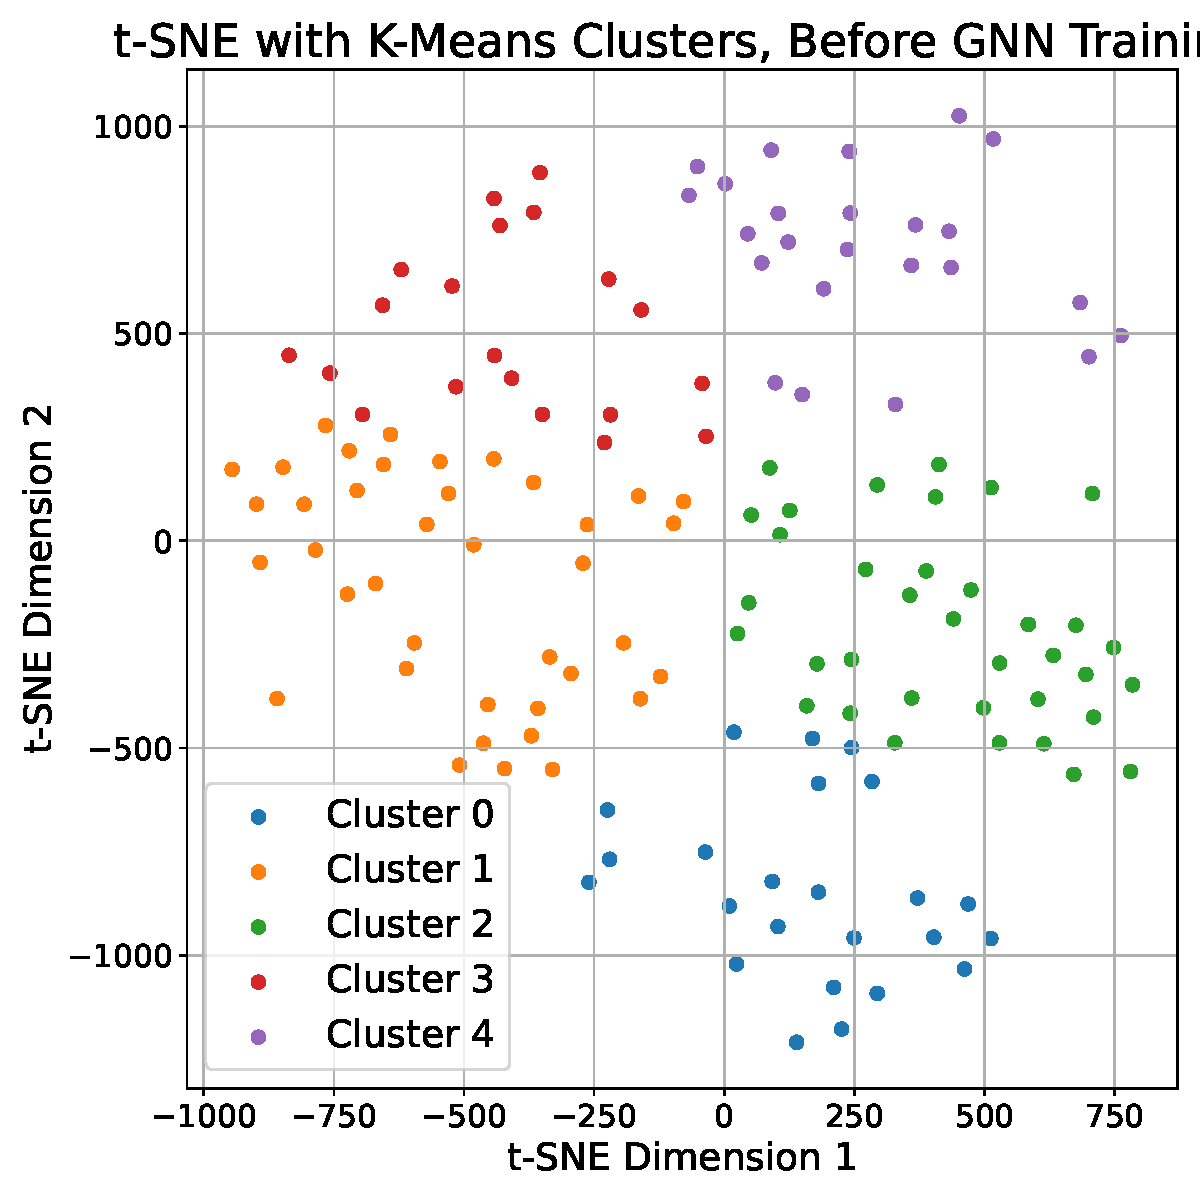
\includegraphics[width=0.66\columnwidth]{figures/t-SNE with K-Means Clusters, Before GNN Training.pdf}
    \caption{5 clusters of CPs before training. Since there are not yet GNN-based vector representations for the CPs, we used the \texttt{cp} node features as vectors.}
    \label{fig:cluster_before_training}
\end{subfigure}

\vspace{1em}

\begin{subfigure}[b]{\columnwidth}
    \centering
    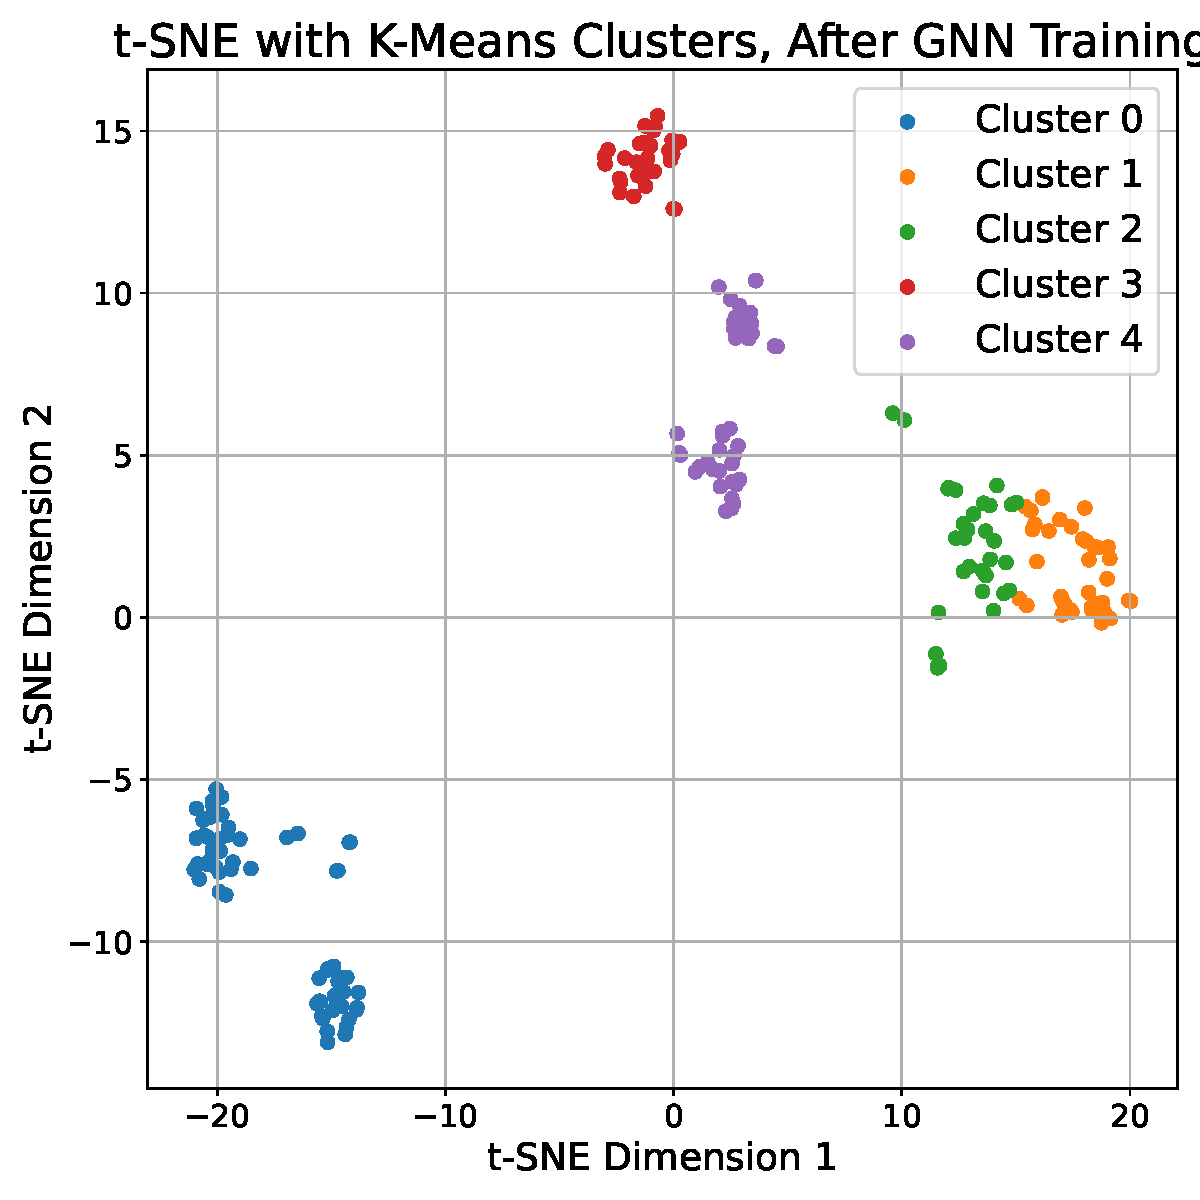
\includegraphics[width=0.66\columnwidth]{figures/t-SNE with K-Means Clusters, After GNN Training.pdf}
    \caption{5 clusters of CPs after training. The vectors used here are the means of the last RGCN layer node representations.}
    \label{fig:cluster_after_training}
\end{subfigure}

\caption{K-means clustering results before and after training, visualized using t-distributed stochastic neighbor embedding (t-SNE) to map high-dimensional vectors into 2D space. $K=5$ was chosen.}
\label{fig:cluster}
\end{figure}


Table~\ref{tab:cluster_stats} presents the performance metrics for each cluster. Notably, Cluster 1 exhibits a higher success rate, suggesting that participants using CPs from this cluster were more likely to rescue the victim. While the other metrics remain important, we emphasize success rate since saving the victim is considered the most critical outcome.

\begin{table}[tb]
    \centering
    \renewcommand{\arraystretch}{1.2}
    \resizebox{\columnwidth}{!}{ % Rescale table
    \begin{tabular}{lcccc}
        \toprule
        \textbf{Cluster} & \makecell{\textbf{Time} \\ \textbf{Elapsed}} & \makecell{\textbf{Remaining} \\ \textbf{Rocks}} & \makecell{\textbf{Victim} \\ \textbf{Harm}} & \makecell{\textbf{Sucess} \\ \textbf{Rate}} \\
        \midrule
        Cluster 0 & 2716 (+120) & 16 (+1.0) & 291 (-14) & 24\% (-3\%) \\
        Cluster 1 & 2133 (-462) & 11 (-3.9) & 318 (+11) & 42\% (+15\%) \\
        Cluster 2 & 2607 (+12) & 11 (-3.2) & 311 (+4) & 36\% (+9\%) \\
        Cluster 3 & 2869 (+273) & 18 (+3.9) & 246 (-60) & 17\% (-11\%) \\
        Cluster 4 & 2629 (+33) & 16 (+1.9) & 355 (+49) & 19\% (-9\%) \\
        \bottomrule
    \end{tabular}
    }
    \caption{Cluster statistics (higher is better for success rate and lower is better for the others.), with differences from the mean in parentheses.}
    \label{tab:cluster_stats}
\end{table}

Table~\ref{tab:cluster_edges} presents the edge types and their frequencies for the CPs in each cluster. Notably, the action edges in Cluster 1 are simpler than those in other clusters, as it contains fewer distinct action types. Of the 78 total edges across all CPs in Cluster 1, the majority involve two consecutive robot actions. This suggests that Cluster 1 not only represents a simpler interaction pattern but also grants greater autonomy to the robot. While robot actions are typically conditioned on human actions, the lower presence of human action edges in this cluster indicates that the robot's behavior is less dependent on human input.

\begin{table}[tb]
    \centering
    \renewcommand{\arraystretch}{1.2}
    \setlength{\tabcolsep}{8pt}
    \begin{tabular}{llc}
        \toprule
        \textbf{Cluster} & \textbf{Edge label} & \textbf{Count (\%)} \\
        \midrule
        \multirow{7}{*}{Cluster 0} 
        & has\_robot\_action\_0 & 62 (55.86\%) \\
        & has\_human\_action\_0 & 30 (27.03\%) \\
        & has\_human\_action\_1 & 8 (7.21\%) \\
        & has\_robot\_action\_2 & 3 (2.70\%) \\
        & has\_robot\_action\_3 & 3 (2.70\%) \\
        & has\_robot\_action\_4 & 3 (2.70\%) \\
        & has\_human\_action\_2 & 2 (1.80\%) \\
        \midrule
        \multirow{3}{*}{Cluster 1} 
        & has\_robot\_action\_1 & 38 (48.72\%) \\
        & has\_robot\_action\_0 & 38 (48.72\%) \\
        & has\_robot\_action\_2 & 2 (2.56\%) \\
        \midrule
        \multirow{6}{*}{Cluster 2} 
        & has\_robot\_action\_1 & 36 (31.30\%) \\
        & has\_robot\_action\_0 & 36 (31.30\%) \\
        & has\_robot\_action\_2 & 31 (26.96\%) \\
        & has\_robot\_action\_3 & 7 (6.09\%) \\
        & has\_human\_action\_1 & 4 (3.48\%) \\
        & has\_human\_action\_2 & 1 (0.87\%) \\
        \midrule
        \multirow{4}{*}{Cluster 3} 
        & has\_human\_action\_0 & 30 (38.46\%) \\
        & has\_robot\_action\_1 & 30 (38.46\%) \\
        & has\_robot\_action\_2 & 16 (20.51\%) \\
        & has\_robot\_action\_3 & 2 (2.56\%) \\
        \midrule
        \multirow{7}{*}{Cluster 4} 
        & has\_human\_action\_0 & 43 (26.22\%) \\
        & has\_robot\_action\_1 & 43 (26.22\%) \\
        & has\_robot\_action\_0 & 42 (25.61\%) \\
        & has\_human\_action\_1 & 20 (12.20\%) \\
        & has\_robot\_action\_2 & 7 (4.27\%) \\
        & has\_robot\_action\_3 & 7 (4.27\%) \\
        & has\_human\_action\_2 & 2 (1.22\%) \\
        \bottomrule
    \end{tabular}
    \caption{Edge label distributions across clusters.}
    \label{tab:cluster_edges}
\end{table}


Considering both performance and structural simplicity, we identified Cluster 1 as the most meaningful set of CPs. It represents a minimal yet effective CP, where the robot operates with greater autonomy while maintaining efficiency. We selected the CP closest to the cluster center (by Euclidean distance) as our final choice, as it best represents the defining characteristics of Cluster 1 and serves as the most typical example of its CP.

Table~\ref{tab:final_cp} presents the final selected CP. Notably, this CP consists of only two consecutive robot actions without any human actions. This suggests that, in this scenario, the robot operates independently, executing its tasks without relying on human input. Compared to other CPs that typically involve human actions, this CP grants the robot greater autonomy in decision-making and task execution. Specifically, this CP directs the robot to move large rocks near the victim. Since only the robot can handle large rocks, this pattern effectively delegates the heavy lifting to the robot while allowing the human to focus on other tasks as they see fit.

\begin{table}[h]
    \centering
    \renewcommand{\arraystretch}{1.2}
    \setlength{\tabcolsep}{5pt}
    \begin{tabular}{lp{5cm}}
        \toprule
        \textbf{Type} & \textbf{Details} \\
        \midrule
        \texttt{situation} & Location: ``Top of rock pile'' \newline
                   Object: ``Large rock'' \\
        \midrule
        \texttt{robot\_action\_0} & Location: ``Top of rock pile'' \newline
                         Object: ``Large rock'' \newline
                         Action: ``Pick up \textless object\textgreater{} in \textless location\textgreater{}'' \\
        \midrule
        \texttt{robot\_action\_1} & Location: ``\textless Right\textgreater{} side of field'' \newline
                         Object: ``Large rock'' \newline
                         Action: ``Drop \textless object\textgreater{} in \textless location\textgreater{}'' \\
        \bottomrule
    \end{tabular}
    \caption{The final selected collaboration pattern (CP).}
    \label{tab:final_cp}
\end{table}

We initialize the robot's memory with the final CP and conduct the MATRX USAR experiment under the same conditions as the previous study, with the only difference being the inclusion of the preloaded memory. We recruited 20 student participants from our university. All experiments were conducted online.\footnote{The experiment involving human participants was approved by our university's ethics committee (ID anonymized).}

\begin{table*}[tb]
    \centering
    \renewcommand{\arraystretch}{1.2}
    \setlength{\tabcolsep}{6pt}
    \resizebox{\textwidth}{!}{ % Ensure table fits within the page width
    \begin{tabular}{c|cc|cc|cc|cc}
    \toprule
    \multirow{2}{*}{Round} 
    & \multicolumn{2}{c|}{\textbf{Time Elapsed}} 
    & \multicolumn{2}{c|}{\textbf{Remaining Rocks}} 
    & \multicolumn{2}{c|}{\textbf{Victim Harm}} 
    & \multicolumn{2}{c}{\textbf{Success Rate}} \\
    & \textbf{\makecell{W/o Memory \\ Initialized}} & \textbf{\makecell{With Memory \\ Initialized}} 
    & \textbf{\makecell{W/o Memory \\ Initialized}} & \textbf{\makecell{With Memory \\ Initialized}} 
    & \textbf{\makecell{W/o Memory \\ Initialized}} & \textbf{\makecell{With Memory \\ Initialized}} 
    & \textbf{\makecell{W/o Memory \\ Initialized}} & \textbf{\makecell{With Memory \\ Initialized}} \\
    \midrule
    1  & 3000 (0)   & 2458 (626)  & 18.2 (6.0)   & 5.8 (8.0)   & 733 (512)  & 160 (320)  & 0.0\% (0.0\%)    & 55.0\% (51.0\%)  \\
    2  & 2677 (604) & 2304 (644)  & 14.5 (13.3)  & 5.3 (8.1)   & 324 (387)  & 255 (349)  & 28.5\% (46.3\%)  & 65.0\% (48.9\%)  \\
    3  & 2410 (707) & 2192 (732)  & 10.4 (13.7)  & 3.5 (7.3)   & 257 (457)  & 465 (589)  & 52.4\% (51.1\%)  & 75.0\% (44.4\%)  \\
    4  & 2475 (699) & 2150 (672)  & 7.9 (9.5)    & 3.5 (7.0)   & 286 (408)  & 160 (201)  & 47.6\% (51.2\%)  & 75.0\% (44.4\%)  \\
    5  & 2493 (722) & 2300 (720)  & 15.9 (12.0)  & 12.0 (9.5)  & 457 (383)  & 470 (508)  & 23.8\% (43.6\%)  & 30.0\% (47.0\%)  \\
    6  & 2590 (630) & 2593 (545)  & 19.0 (9.6)   & 14.0 (7.7)  & 476 (648)  & 520 (393)  & 4.7\% (21.8\%)   & 15.0\% (36.6\%)  \\
    7  & 2503 (555) & 1994 (784)  & 15.5 (11.9)  & 17.1 (6.9)  & 310 (319)  & 880 (635)  & 23.8\% (43.6\%)  & 5.0\% (22.4\%)   \\
    8  & 2558 (545) & 2448 (660)  & 14.5 (11.4)  & 12.5 (6.9)  & 535 (701)  & 1190 (679) & 25.0\% (44.4\%)  & 10.0\% (30.8\%)  \\
    \midrule
    \textbf{Overall} 
    & 2588 (613)  & \textbf{2305 (686)}  
    & 14.5 (11.4) & \textbf{9.2 (9.1)}  
    & \textbf{422 (504)}   & 513 (583)  
    & 25.7\% (43.9\%)  & \textbf{41.3\% (49.4\%)}  \\
    \bottomrule
    \end{tabular}
    }
    \caption{Comparison of the robot without initialized memory and the robot with initialized memory. 
    Values are presented as \textit{Average (std)}, where standard deviation is in parentheses. 
    Success rate is reported as a percentage (\%), where higher is better; lower is better for the other metrics. 
    Both the robot without memory and the robot with initialized memory were evaluated using 20 samples (participants) each. Better values for each metric are shown in \textbf{bold}.}
    \label{tab:comparison} 
\end{table*}

Table~\ref{tab:comparison} shows that the robot with initialized memory consistently outperforms the one without it, except in ``victim\_harm,'' likely due to accidental rock falls when removing large rocks. Statistical analysis confirms this improvement is significant: with $n = 8 \times 20 = 160$ observations per group, the success rate increased from 25.7\% to 41.3\% (a 60.7\% relative improvement), with $t(318) = 2.986$, $p = 0.0015$ (one-tailed), and Cohen's $d = 0.334$. The 95\% confidence interval [5.3\%, 25.9\%] excludes zero, confirming the reliability of our findings. Notably, the most significant improvement occurs in Round 1, where participants are still unfamiliar with the environment. Since the robot begins with prior knowledge from past interactions, it can immediately engage in effective collaboration, providing a smoother start for the human-robot team.

Interestingly, the selected CP (Table~\ref{tab:final_cp}) does not reference the ``Brown rock,'' which only appears in later rounds (Rounds 5–8). Despite this, the robot with initialized memory continues to facilitate better performance in most of the rounds, except 7 and 8. This suggests that the chosen CP captures a generally effective collaboration strategy, enabling the robot to adapt even in scenarios it has not explicitly encountered before.

\section{Related Work}
\label{sec:related_work}

Our work builds on several research strands, including human-like memory in agents, KG representations for complex relational data, graph neural networks for structured learning, and human-robot collaboration in challenging environments such as urban search and rescue (USAR). In this section, we discuss these lines of research and position our contribution in relation to existing approaches.

Our work is inspired by the concept of agents' episodic memory, where past experiences are stored and reactivated to guide future actions. Early approaches, drawing on cognitive science, used symbolic and rule-based systems to mimic human memory functions in agents. More recent methods, such as those by Parisotto et al.~\cite{pmlr-v70-pritzel17a} and Rebuffi et al.~\cite{chaudhry2019efficientlifelonglearningagem}, employ deep learning to capture and encode complex interaction patterns, enabling agents to both recall and generalize from previous experiences. We extend these ideas by representing episodic memories as KGs, providing a structured format that captures performance metrics and contextual details of human-agent collaborations, thereby facilitating more effective retrieval and application of prior experiences in challenging scenarios.

Kim et al.~\cite{https://doi.org/10.48550/arxiv.2204.01611,Kim_Cochez_Francois-Lavet_Neerincx_Vossen_2023} adopted a cognitive science-inspired approach to develop a human-like memory system. Their agents incorporate both episodic and semantic memory components. In their framework, episodic memory captures the agent's direct experiences, while semantic memory encompasses general factual knowledge—information that can be acquired through learning or provided by human experts.

Self-supervised learning is central to modern large language models like BERT~\cite{DBLP:journals/corr/abs-1810-04805} and GPT-3~\cite{DBLP:journals/corr/abs-2005-14165}, which capture rich contextual information from unlabeled data by reconstructing or predicting missing parts (e.g., via masked language modeling or next-token prediction). Similarly, self-supervised techniques in graph neural networks enable the extraction of meaningful embeddings from inherently unlabeled node data. These learned representations, which capture structural and relational nuances, can then be leveraged for downstream tasks such as clustering. In our work, we use self-supervised graph learning to derive robust representations of episodic memory KGs, facilitating efficient clustering of CPs.

Collaborative learning in human-robot teams has emerged as a pivotal factor for enabling mutual adaptation and shared understanding in dynamic task environments. Baxter et al.~\cite{Baxter2017RobotEP} demonstrated that personalized interactions between robots and human learners can significantly enhance educational outcomes, setting the stage for further exploration into adaptive team behaviors. Building on this, Belpaeme et al.~\cite{Belpaeme2018} provided comprehensive guidelines for designing social robots that effectively serve as second language tutors, emphasizing the importance of interactive, adaptive strategies. Complementing these efforts, Nikolaidis et al.~\cite{Nikolaidis} investigated mutual adaptation in collaborative tasks, offering experimental evidence that both humans and robots benefit from continuous reciprocal learning. Moreover, Holstein et al.~\cite{Holstein} introduced a conceptual framework for human-AI hybrid adaptivity in educational settings, highlighting how effective communication and adaptive strategies can jointly drive collaborative learning. These studies collectively underscore the potential of leveraging mutual adaptation to foster robust and resilient human-robot partnerships.

Collaborative work has further enriched our understanding of human-robot co-learning. For instance, Shafti et al.~\cite{DBLP:journals/corr/abs-2003-01156} demonstrated effective human-robot collaboration through reinforcement learning in real-world scenarios, while Wenskovitch et al.~\cite{WenskovitchInteractiveAD} addressed the challenge of transparency in interactive AI systems, emphasizing the need for interpretable decision-making in collaborative settings. Moreover, Gao et al.~\cite{gao} explored personalized human-robot co-adaptation in instructional environments, highlighting how tailored interaction strategies can enhance mutual learning. These studies complement the aforementioned works by providing diverse perspectives on designing adaptive, communicative, and transparent systems for robust human-robot collaboration.

Recent work by van Zoelen et al.~\cite{10.1145/3434074.3446354,vanZoelen2021,vanZoelen2022} systematically identified recurring interaction patterns in human-robot co-adaptation using the MATRX USAR environment. Their study distinguishes between stable situations and sudden adaptations, offering a behavioral framework that captures the dynamics of mutual adaptation in team settings. These insights underscore the context-dependent nature of co-learning and provide a valuable foundation for designing systems that support effective human-robot interactions. Building on this work, our approach integrates KG-based representations of episodic memory with self-supervised graph learning, enabling efficient clustering and retrieval of these interaction patterns to enhance team-level performance in dynamic environments.


\section{Conclusion}
\label{sec:conclusion}


We showed that initializing a USAR robot with a single collaboration pattern stored as a knowledge‑graph episodic memory, learned by self‑supervised relational GNNs, can boost human–robot teamwork. In 160 MATRX trials the seeded robot raised victim‑rescue success from 25.7\% to 41.3\% and cut average task time by 283s. However, the study also comes with some limitations. It was limited to simulation with 20 student participants, one CP drawn from the best cluster, and a domain‑specific ontology; budget constraints precluded testing other cluster exemplars, and victim‑harm sometimes increased when the robot moved heavy debris. Future work will pursue online growth / pruning of the episodic memory and transfer to other collaborative domains.

\bibliographystyle{ieeetr}
\bibliography{references}



\end{document}
